\subsection{Database}
Since the web application requires a database to store information about users, questions, sessions, courses and more, a set of files were created to get, insert and update the information. The database is designed around features needed for the application. It was also created for scalability in mind with for example the possibility to add other OAuth/OpenID connect possibilities in the future. There are five scripts associated with the database, where get, insert and update functions have been separated into their own scripts. One script is connecting the get, insert and update scripts making it easier to import and use the database functions in other scripts. There is also a script which will run every time the server starts. This script makes sure that every table is created and have the correct column names. It is also the script that inserts default values such as question types and the anonymous user.
\begin{figure}[H]
    \centering
    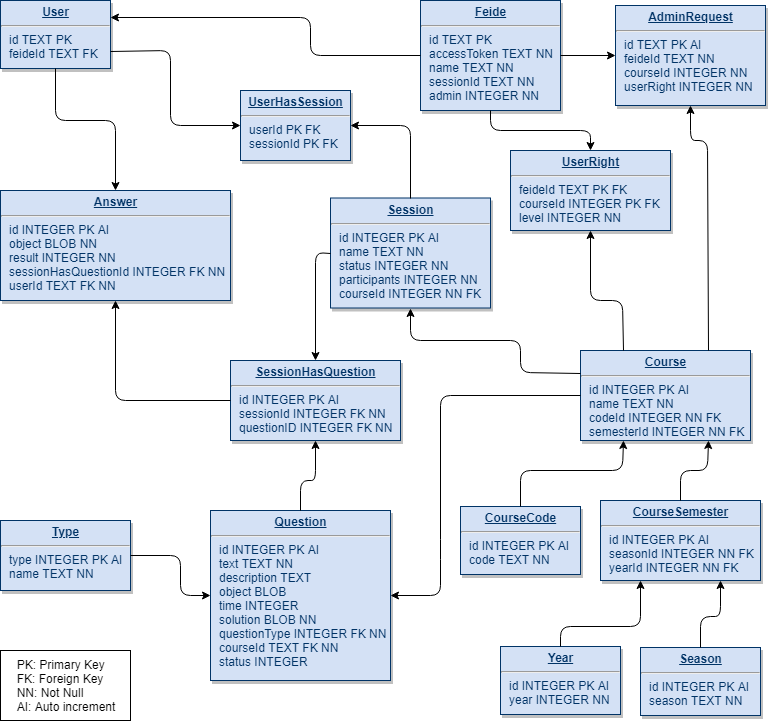
\includegraphics[width=\linewidth]{diagrammer/databaseSchema.png}
    \caption{This is the database schema used for Interaktiv Undervisning}
    \label{fig:dbSchema}
\end{figure}
The table "User" has the anonymous user with user id 1. When an anonymous user answers a question, the answer is linked to that user, no matter who answered. Feide information is in its own table, this makes it easy to add more types of login services, e.g., Facebook, Google, and more. When an admin adds a question to a session, it is linked in its own table called "QuestionHasSession". This is to ensure that a question can be linked to more than one session or multiple times in the same session. The answers are also linked to the "QuestionHasSession" table, making sure that the answers shown to admins are only for that question in that session and not the total answers statistics for the question in general. Sessions are linked to a course. A course contains information about the course code and semester, enabling the option to separate sessions from each semester. Questions are linked to the course id, but admins do have the option to copy questions from one course to another in the question dashboard.